%%%%%%%%%%%%%%%%%%%%%%%%%%%%%%%%%%%%%%%%%%%%%%%%%%%%%%%%%%%%%%%%%%%%%%%%%%%%%%%
\section{The search for magnetic monopoles}
%\section{The search for magnetic monopoles (and other animals)}
\label{sec:search}
%%%%%%%%%%%%%%%%%%%%%%%%%%%%%%%%%%%%%%%%%%%%%%%%%%%%%%%%%%%%%%%%%%%%%%%%%%%%%%%
%%=============================================================================
%\subsection{The state of play}
%\label{sec:stateofplay}
%%=============================================================================
At the time of writing,
no experimental evidence for the existence of magnetic monopoles has been
recorded in the scientific literature.
While \ac{MoEDAL} hopes to change all of that with results from the \ac{LHC}'s
$13 \TeV$ proton-proton collisions, for now we can only look at the results
from all of the experiments that have tried so far.
These searches broadly fall into two categories:
looking for human-made monopoles from particle colliders (``farmed'')
and
looking for monopoles produced by Nature (``free-range'')
that would be found in cosmic rays that hit the Earth.

%
\begin{table}[htbp]
  \centering
  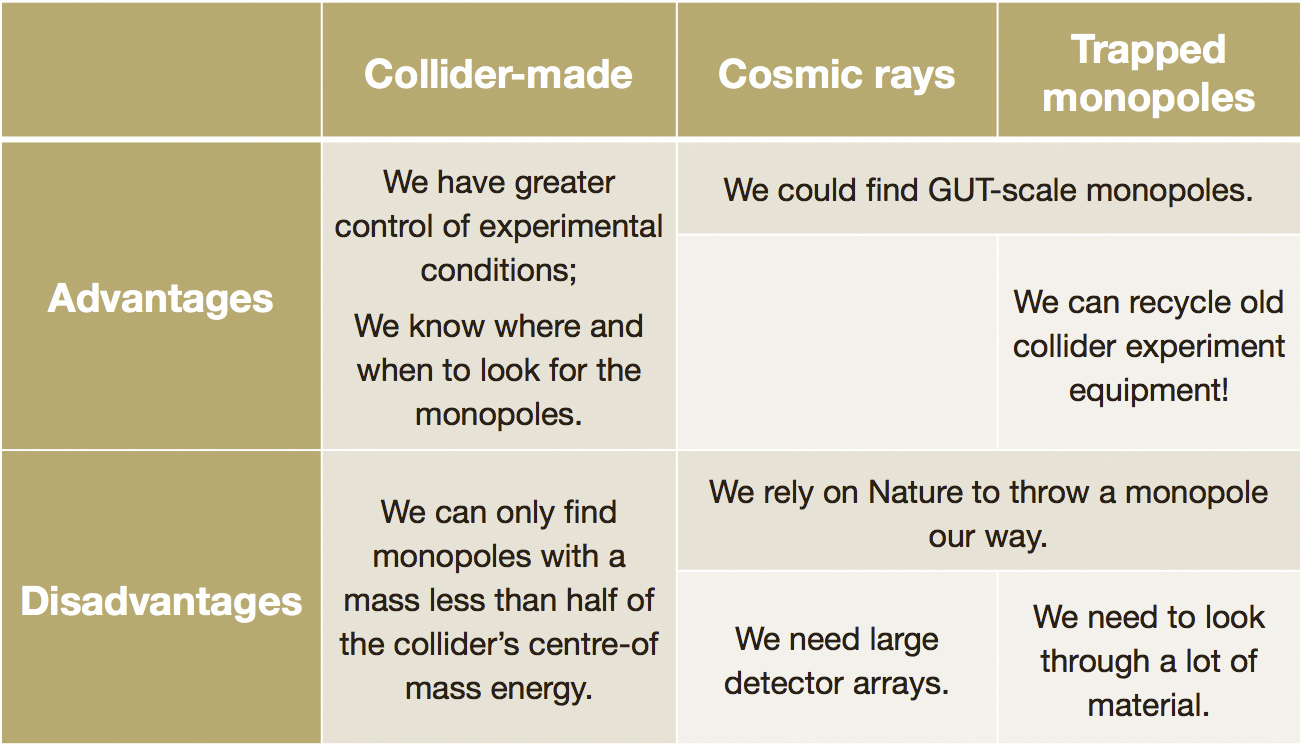
\includegraphics[width=0.75\textwidth]{assets/images/search-table/search-table.jpg}
  \caption[Monopole search strategies]
  {\label{tab:searchstrategies}The advantages and disadvantages of the different search %
strategies employed to find experimental evidence for magnetic monopoles.}
\end{table}
%

The advantage of the former approach is that we would know where and
(roughly) when the monopole-antimonopole pair was produced;
we have far more knowledge of the experimental conditions.
We are, however, limited by the centre-of-mass energy of the
collider in question.
Cosmic ray-based monopole searches rely on catching a ``free-range''
monopole by chance -- and the odds aren't great -- but are capable of
finding the sort of monopole required by \acp{GUT} which
are far beyond what colliders could ever hope to produce.

An excellent summary all the results to-date is presented in
Section 5 of L. Patrizii and M. Spurio’s review paper,
``{\em Status of Searches for Magnetic Monopoles}''~\cite{Patrizii2015}.
You can read the arXiv preprint of this paper
\href{http://arxiv.org/abs/1510.07125}{here}\footnote{%
See \href{http://arxiv.org/abs/1510.07125}{http://arxiv.org/abs/1510.07125}} for free.
The paper also contains sections on monopole theory,
energy losses, experimental methods and what the future holds for monopole
searches (including a shout-out to MoEDAL, of course!) -- so it's well worth
a read -- but some very brief summaries are provided below for convenience.


%=============================================================================
\subsection{Collider-based searches}
\label{sec:searchescollider}
%=============================================================================
{\em See Section 5.1 of~\cite{Patrizii2015} for further information and
full references.}

Magnetic monopoles have been looked for whenever a particle collider has
opened a new energy frontier.
For electron-positron collisions,
the latest results have come from experiments using the
\ac{LEP} collider (for which the LHC's tunnel was originally constructed).
%
\href{http://opal.web.cern.ch/Opal/}{OPAL} (see Figure~\ref{fig:opal})
and \acs{MODAL} (a forerunner of MoEDAL) experiments used both the active 
detector systems and \ac{NTD} arrays to spot monopole-antimonopole pairs.  
\acp{NTD} around beam interaction points were also used at the TRISTAN 
ring at \acs{KEK} (Japan), PETRA at DESY (Germany), and \acs{PEP} at
\acs{SLAC} (US).
Likewise, the best proton-antiproton results have come from Fermilab's
D0, \acs{CDF}, and FNAL E710 experiments using similar techniques.

%
\begin{figure}[htbp]
  \centering
  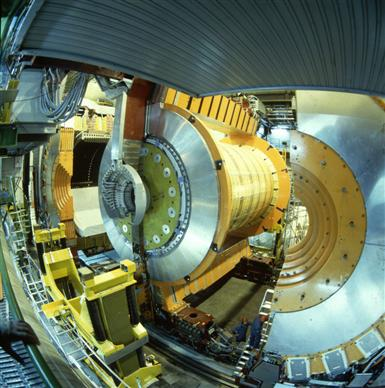
\includegraphics[width=0.6\textwidth]{assets/images/opal/opal.jpg}
  \caption[The OPAL experiment at CERN's LEP Collider]
  {\label{fig:opal}The \acf{OPAL} detector at Interaction Point 6 (IP6), %
which has set some of the most stringent limits on monopole production for %
electron-positron colliders. %
Image credit: \href{https://commons.wikimedia.org/wiki/File:OPAL.jpg}{CERN/Wikimedia Commons}; %
please refer to their terms of use regarding licensing/re-use of this image.}
\end{figure}
%

The best proton-proton results are from the \ac{LHC}'s \ac{ATLAS} and \ac{CMS}
detectors at 8 \ac{TeV}, though these are based on active (electronic) 
detectors. \ac{MoEDAL} will ultimately produce the best \ac{NTD}-based
searches for magnetic monopoles -- and you could part of this with \ac{IRIS}!

%=============================================================================
\subsection{Cosmic ray-based searches}
\label{sec:searchescosmicray}
%=============================================================================
{\em See Sections 5.2 and 5.3 of~\cite{Patrizii2015} for further
information and full references.}

Searches for monopoles in cosmic rays typically need to take place in 
underground laboratories, where backgrounds from cosmic muons or background 
radiation can be minimised.
The best results so far come from the \acf{MACRO} observatory at the
Laboratori Nazionali del Gran Sasso, Italy (Figure~\ref{fig:macro}).
%
Using a combination of liquid scintillation detectors, streamer tubes, 
and \acfp{NTD} -- the largest ever deployed -- \ac{MACRO} saw only
ever saw a ``dummy'' monopole event (used to test the detection systems).
It completed its experimental run in 2001.

%
\begin{figure}[htbp]
  \centering
  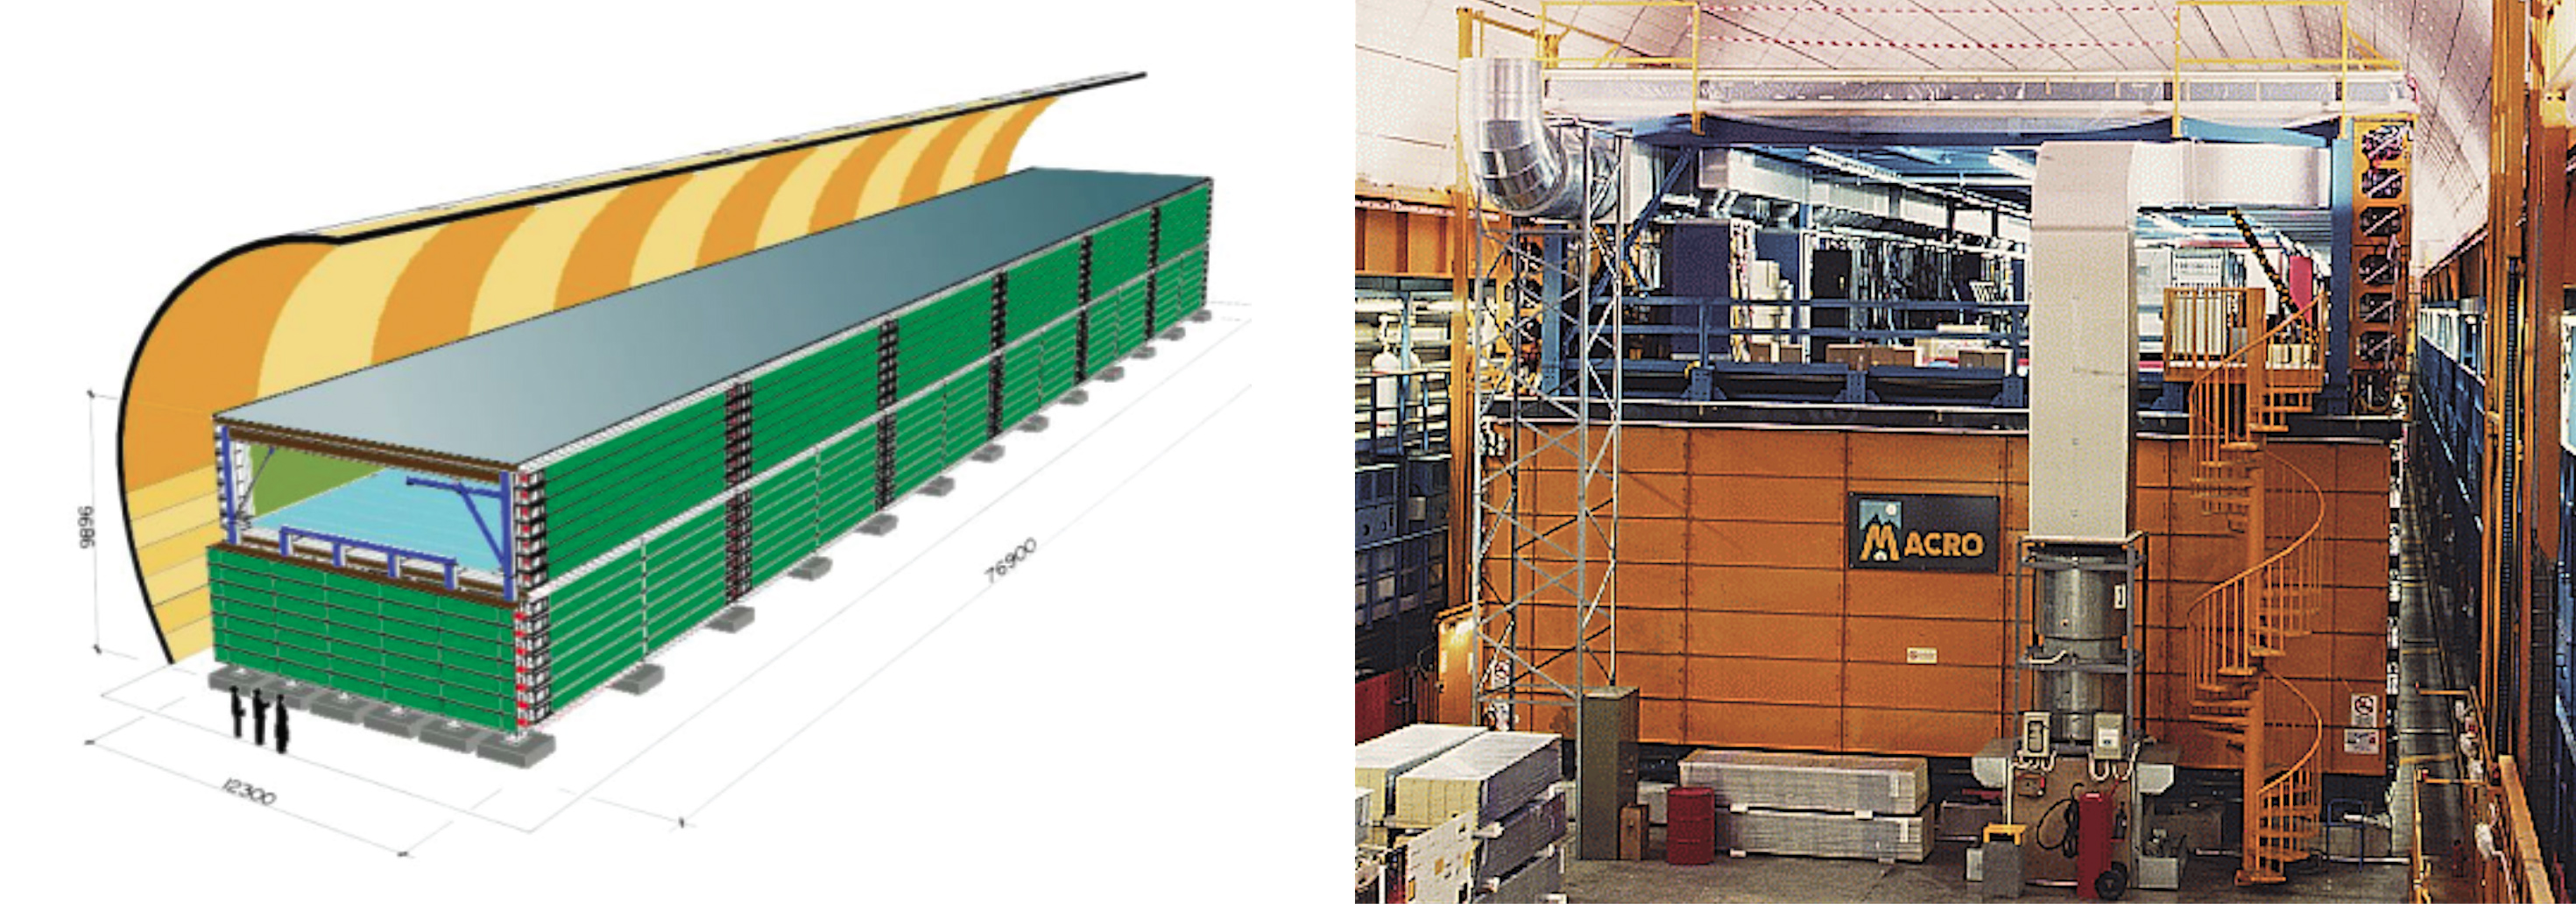
\includegraphics[width=1.0\textwidth]{assets/images/macro/macro.jpg}
  \caption[The MACRO experiment]
  {\label{fig:macro}The \acs{MACRO} (Monopole, Astrophysics and Cosmic Ray) %
observatory at the Laboratori Nazionali del Gran Sasso, Italy. %
Left -- artist's impression; %
right -- the detector itself. %
Image credit: \href{http://arxiv.org/abs/0707.1691}{The MACRO Collaboration}; %
please contact them regarding licensing/re-use of this image.}
\end{figure}
%

If cosmic ray backgrounds can be accounted for, other types of searches 
are possible.  The \ac{SLIM} experiment (Figure~\ref{fig:slim}) used
\acp{NTD} at an altitude of 5.2km exposed for just over four years.
Searches for relativistic monopoles have been conducted with neutrino 
telescopes like \acs{AMANDA}, \acs{ANTARES}, and IceCube 
(See Section 5.2.2 of~\cite{Patrizii2015} for more information).
These rely on the huge showers of Cerenkov light that monopoles would 
produce in the Antarctic ice, but due to the cosmic backgrounds can only 
look for candidates have come up all the way through the Earth.  
Again, these have seen nothing and the best result remains that of the 
\ac{MACRO} experiment.

%
\begin{figure}[htbp]
  \centering
  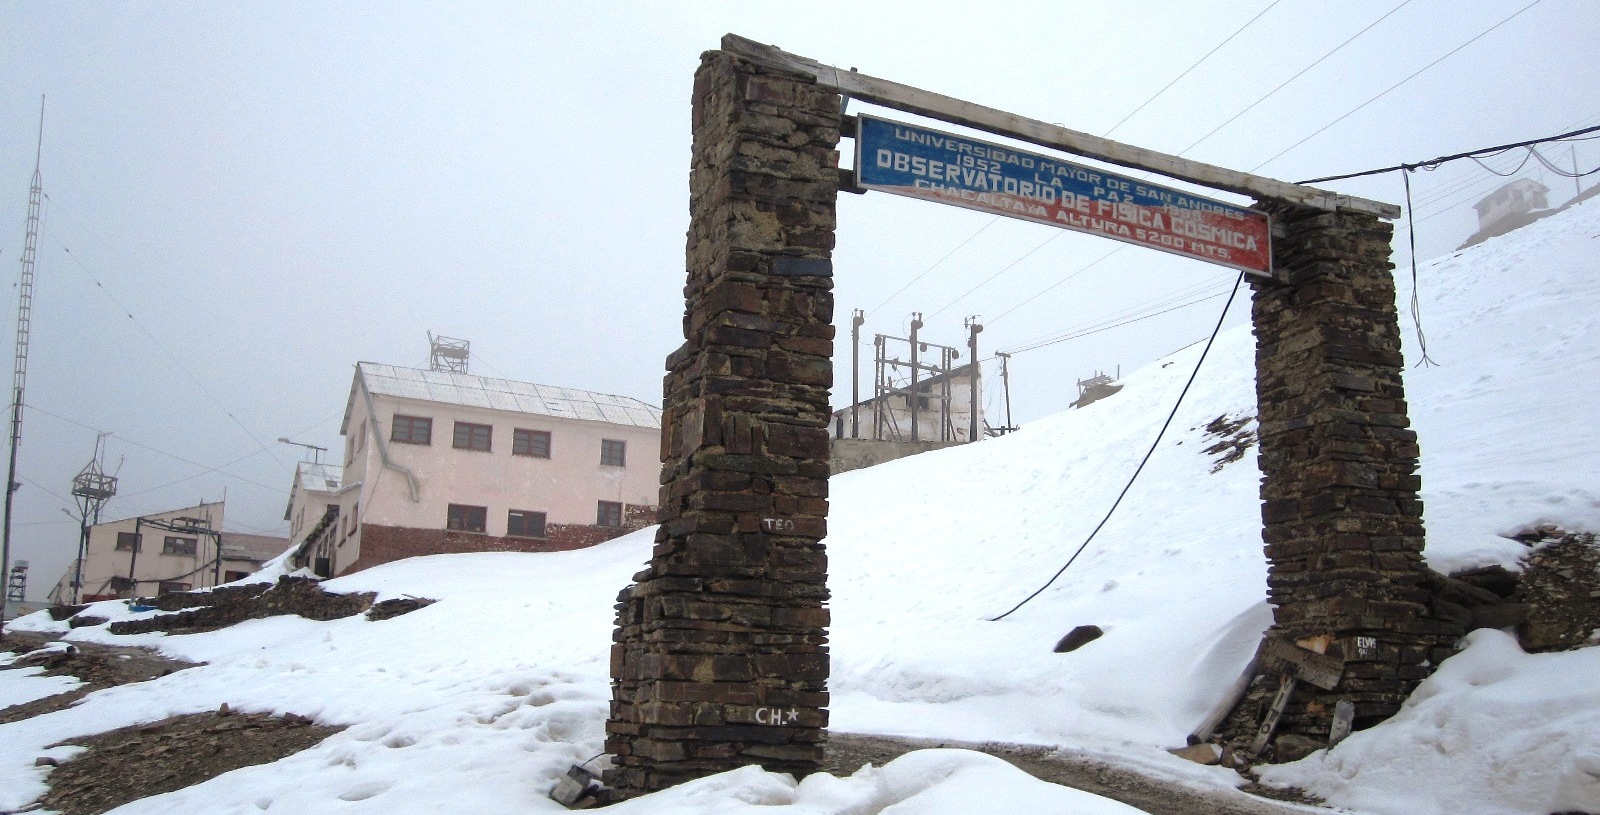
\includegraphics[width=1.0\textwidth]{assets/images/slim/slim.jpg}
  \caption[The Chacaltaya Astrophysical Observatory]
  {\label{fig:slim}The Chacaltaya Astrophysical Observatory, home of the %
\acs{SLIM} (Search for LIght magnetic Monopoles) experiment~\cite{SLIM2008a, SLIM2008b} %
which looked for magnetic monopoles in cosmic rays at an altitude of 5,230m above sea level. %
Image credit: \href{https://commons.wikimedia.org/wiki/File:Chacaltaya\_Astrophysical\_Observatory\_\%2804\%29.JPG}{Wikimedia Commons}; %
please refer to their terms of use them regarding licensing/re-use of this image.}
\end{figure}
%


%=============================================================================
\subsection{Trapped monopoles}
\label{sec:searchestrapped}
%=============================================================================
{\em See Sections 5.1 and 5.4 of~\cite{Patrizii2015} for further information
and full references.}

The third category of search takes a slightly different approach. 
Rather than record the tracks left by a magnetic monopole, 
one can try looking for monopoles in sample of material that might slow down 
a monopole enough to stop it and trap it.  
The trick is picking the right material, but the technique can be applied 
to both collider-produced and cosmic ray monopoles.  
For example, the H1 experiment at \acs{DESY}, Germany cut up 60cm of its 
aluminium beam pipe into pieces and scanned them with a \acf{SQUID}
to look for magnetic monopoles produced in the electron-proton collisions 
of \acs{HERA} (see Figure~\ref{fig:h1}).
Likewise, work has been carried out with material from the D0 and \acs{CDF}-based
Tevatron experiments (i.e. proton-antiproton collisions). 
Cosmic (i.e. \ac{GUT}-scale) monopoles have been looked for in terrestrial, 
lunar and meteoric material using similar methods.

%
\begin{figure}[htbp]
  \centering
  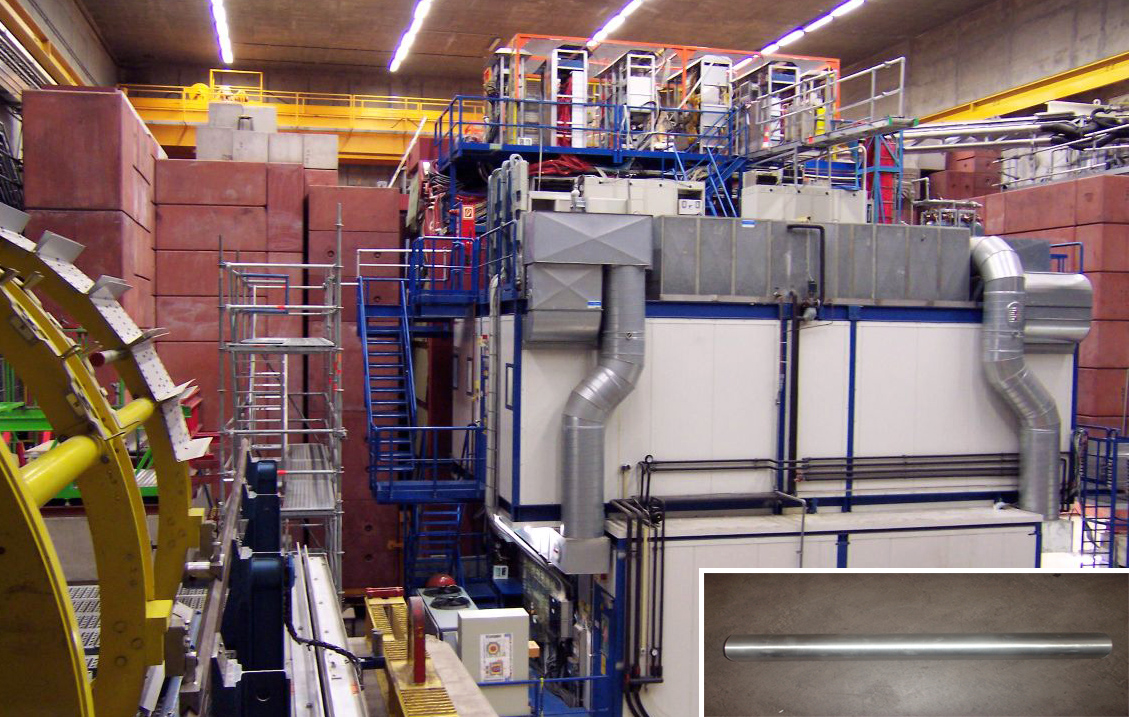
\includegraphics[width=1.0\textwidth]{assets/images/h1/h1.jpg}
  \caption[The H1 detector at DESY, Germany]
  {\label{fig:h1}The H1 detector at \ac{DESY}, Germany. %
Inset (bottom-right): a 60cm section of the H1 beam pipe used between 1994 %
and 1997 in a trapped monopole search. %
Image credit: \href{https://en.wikipedia.org/wiki/File:H1\_detector.jpg}{G. Brandt/Wikimedia Commons}; %
please refer to their terms of use regarding licensing/re-use of this image.}
\end{figure}
%

\ac{MoEDAL} continues this tradition with its \acf{MMT} subdetector (Section~\ref{sec:mmt}), 
which consists of hundreds of kilograms of aluminium bars placed within the \acs{LHCb} cavern.
These can then be removed and replaced during the \ac{LHC} shutdowns to allow \acs{SQUID}
scans of the bars to be made before the \ac{LHC} finishes running and the \ac{ATLAS} and \ac{CMS}
detectors are decommissioned.
